\documentclass{article}
\usepackage{ifxetex}
\ifxetex
  \usepackage{fontspec}
\else
  \usepackage[T1]{fontenc}
  \usepackage[utf8]{inputenc}
  \usepackage{lmodern}
  \usepackage{float}
  \usepackage{graphicx}
  \usepackage{morefloats}
  \usepackage{wrapfig}
  \usepackage{babel}
  \usepackage{enumerate}
\fi
\begin{document}
\begin{titlepage}
\begin{center}
    \vspace*{-1in}
    \begin{figure}[htb]
    \begin{center}
    
\includegraphics[width=8cm]{escudo-gde-trans.png}
    \end{center}
\end{figure}
\begin{center}
LICENCIATURA EN FÍSICA \\
\vspace*{0.15in}
DEPARTAMENTO DE FÍSICA \\
\vspace*{0.6in}
\begin{large}
FÍSICA COMPUTACIONAL 1 \\
\end{large}
\vspace*{0.2in}
\rule{80mm}{0.1mm}\\
\vspace*{0.1in}
\begin{large}
\textbf{Reporte 7\\ }
\end{large}
\vspace*{0.3in}
\begin{large}
Alumna: \\
\vspace*{0.1in}
Brambilla Zamorano Fátima Fernanda\\
\end{large}
\vspace*{0.3in}
\rule{80mm}{0.1mm}\\
\vspace*{0.1in}
\begin{large}
Fecha: \\ 16/03/18\\
\end{large}
\end{center}
\end{center}
\end{titlepage}

\section{Coupled spring equations}
\subsection{Introducción}
Los métodos clásicos para empezar ecuaciones diferenciales están cambiando rápidamente por técnicas de solución para una variedad de ecuaciones diferenciales, para enfatizar sistemas y aspectos más cualitativos de la teoría de ecuaciones diferenciales ordinarias. En particular, hay un enfasís en las ecuaciones no lineales, debido en gran medida a la amplia disponibilidad de algoritmos númericos altamente poderosos, y a capacidades gráficas que vienen con sistemás algebráicos computacionales, como lo son \textit{Mathematica} y \textit{Maple}.
En el siguiente articulo se presentará un viejo problema que ahora se utiliza en los libros de texto. Se trata del problema de dos resortes y dos masas atados en serie, y colgando del techo. Bajo la suposición de que que las fuerzas restauradoras se comportan de acuerdo a la Ley de Hooke, este problema de dos grados de libertad esta modelado por dos parejas de ecuaciones diferenciales de segundo orden.

\subsection{The coupled spring model}
El modelo consiste en dos resortes y dos masas. Un muelle, que tiene una constante elástica k1, esta atado al techo y a un peso con masa m1 en su parte inferior.
A este peso, se le ata un segundo resorte de constante elástica k2, y así mismo este resorte tiene en su parte inferior atado un peso de masa m2. Como se puede ver en la siguiente figura.

\begin{figure}[htb]
    \begin{center}
    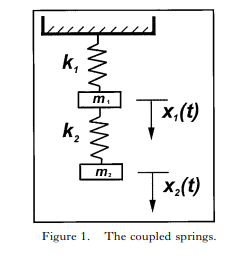
\includegraphics[width=6cm]{Figura1.PNG}
    \end{center}
\end{figure}

Permitiendo al sistema volver a su posición de equilibrio, medimos el desplazamiento del centro de masa de cada peso desde el equilibrio en función del tiempo, y denotamos estas mediciones como x1(t), y x2(t) respectivamente.

\subsubsection {Asumiendo la Ley de Hooke}
Bajo la suposición de pequeñas oscilaciones, las fuerzas de restauración son de la forma: -k1L1, y -k2L2, donde L1 y L2 son las elongaciones (o compresiones) de los dos resortes. Dado que la masa superior esta atada a ambos resortes, hay dos fuerzas restauradoras actuando sobre ella: una hacía arriba de la forma -k1x1, ejercida por la elongación (o comprensión) x1 del primer resorte; y otra hacía arriba de la forma -k2(x2 - x1) de la resistencia del segundo resorte a ser comprimido (o elóngado) por la cantidad (x2 - x1). La segunda masa solo "siente" la fuerza restauradora de la elongación (o compresión) del segundo resorte.
Asumiendo que no hay fricción en el sistema, entonces la ley de Newton implica que las dos ecuaciones que representan el movimiento de las dos masas son las siguientes:
\begin{equation}
m1x'1 = -k1x1 - k2*(x2-x1)
\end{equation}
\begin{equation}
m2x'2 = - k2*(x2-x1)
\end{equation}

Sin embargo, estas ecuaciones no nos son de mucha ayuda para resolver el sistema, por lo que después de un largo procedimiento para obtener un par de ecuaciones que nos sean útiles, llegamos al siguiente sistema:

\begin{equation}
x'1 = u
\end{equation}
\begin{equation}
u' = (-k1x1 - k2(x1 - x2))/m1
\end{equation}
\begin{equation}
x'2 = v
\end{equation}
\begin{equation}
v' = (-k2(x2 -x1))/m2
\end{equation}

\subsection {Adding nonlinearity}
Si asumimos que la fuerzas restauradoras no son lineares, lo cual es cierto para la mayoría de las vibraciones largas,podemos modificar el modelo de acuerdo al sistema. Más que asumir que la fuerza restauradora es de la forma -kx (Ley de Hooke), supongamos que tomamos la fuerza de restauración de la forma:
\begin{figure}[H]
    \includegraphics[width=0.15\textwidth]{Captura.PNG}
    \centering
    \label{Cod}
\end{figure}
Entonces nuestro modelo esta descrito por las siguientes ecuaciones:
\begin{figure}[H]
    \includegraphics[width=1\textwidth]{Captura1.PNG}
    \centering
    \label{Cod}
\end{figure}
El rango de movimiento de los modelos no lineales es bastante más complicado que el modelo lineal. Además, aparecen más preguntas cuando se resuelven estas ecuaciones. Los métodos númericos pueden resolver estos problemas para intervalos de tiempo amplios.

\subsection {Adding forcing}
Es en realidad algo sencillo añador una fuerza exterior al modelo. Suponga que asumimos una fuerza simple y senoidal de la forma \textit{Fcoswt}. En ese caso, el modelo se convierte en el siguiente
\begin{figure}[H]
    \includegraphics[width=1\textwidth]{Captura2.PNG}
    \centering
    \label{Cod}
\end{figure}
El rango de movimiento para los modelos no lineales es bastante amplio. Por ello, podemos esperar encontrar soluciones múltiples para el sistema, ya sea que estén en sistemas de dos incognitas (o más), o no, soluciones periodicas que comportan el periodo con la fuerza (llamadas soluciones armónicas), y soluciones que son periodicas del período de un múltiplo del periodo de conducción (llamadas soluciones subarmonicas), y soluciones de periodos estáticos y constantes. Las condiciones bajo las cuales estos movimientos ocurren, no son fáciles de declarar.

\section{Procedimiento}
Para resolver el sistema de manera númerica, nos apoyamos en \textit{Jupyter Lab}, que es algo diferente al notebook, donde habíamos estado trabajando anteriormente, no obstante, al estar ya familiarizados con su empleo, no hubo ni un problema al empezar a trabajar en la plataforma mencionada.
En primer lugar, definimos un vector con las ecuaciones previas, para poder trabajar los ejemplos que más adelante se nos pedía resolver y comparar con los resultados mostrados en el archivo de texto.
\begin{figure}[H]
    \caption{Celda 1}
    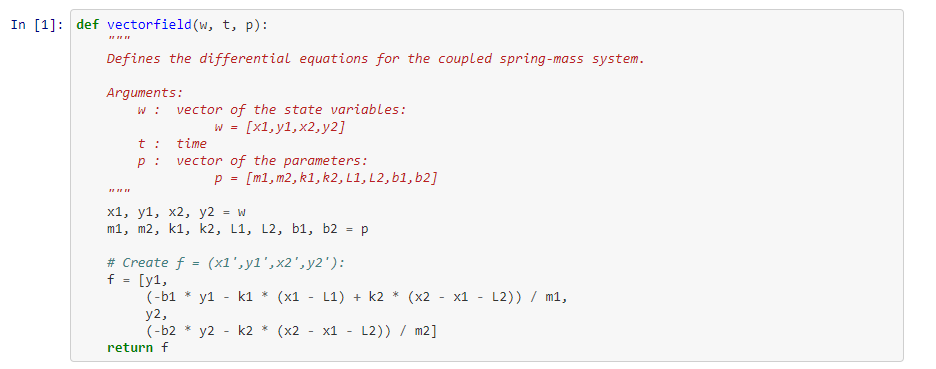
\includegraphics[width=1\textwidth]{Celda1.PNG}
    \centering
    \label{Cod}
\end{figure}

Después de definir el vector, el cual podía reutilizarse para cada uno de los ejemplos que se resolverían más adelante, en una segunda celda se pusieron las condiciones iniciales y los datos indicados en el ejemplo 3.1 del archivo de texto. En esta celda también se escribió el siguiente código, para que el programa pudiera resolver el problema:
\begin{figure}[H]
    \caption{Celda 2}
    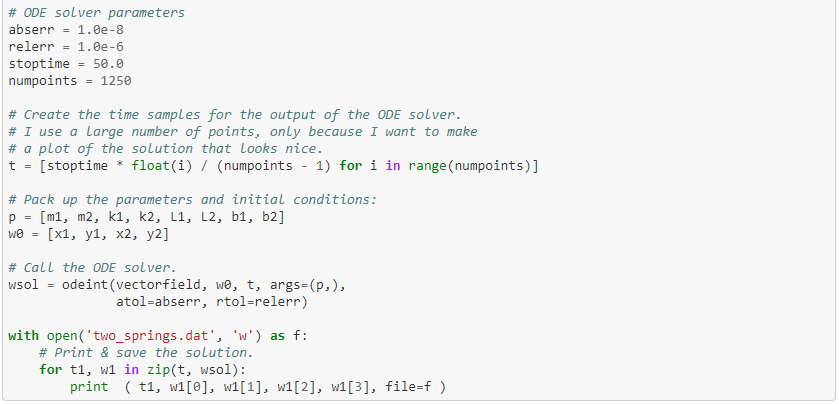
\includegraphics[width=1\textwidth]{Celda2.PNG}
    \centering
    \label{Cod}
\end{figure}
En la tercera celda, se importaron diferentes bibliotecas para la creación de gráficas, y el guardado de archivos de datos o imágenes, y se escribo el código para crear la primera gráfica, como se muestra en la siguiente figura.
\begin{figure}[H]
    \caption{Celda 3}
    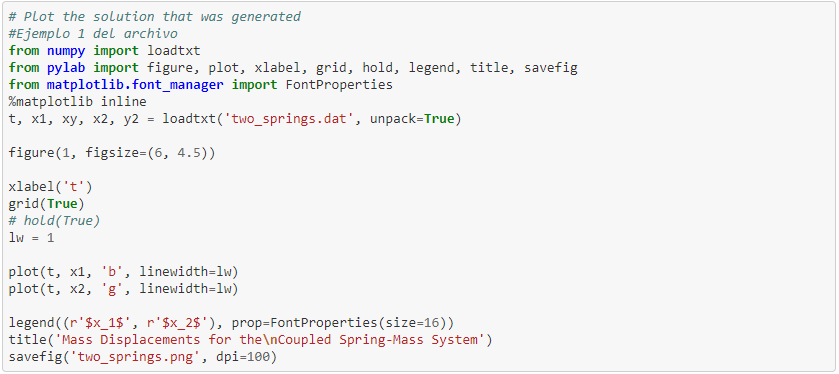
\includegraphics[width=1\textwidth]{Celda3.PNG}
    \centering
    \label{Cod}
\end{figure}
Las tres figuras anteriores muestran el código base que se uso para cada ejemplo del texto, de modo que a continuación se mostraran los resultados obtenidos, así como los fragmentos de código que se hayan usado a parte para cada ejemplo.

La siguiente figura muestra los cambios hechos al código mostrado en la primera celda, y dicha modificación fue hecha para añadir efectos de fuerzas no lineales al problema, así como fuerzas externas al sistema:
\begin{figure}[H]
    \caption{Celda 3}
    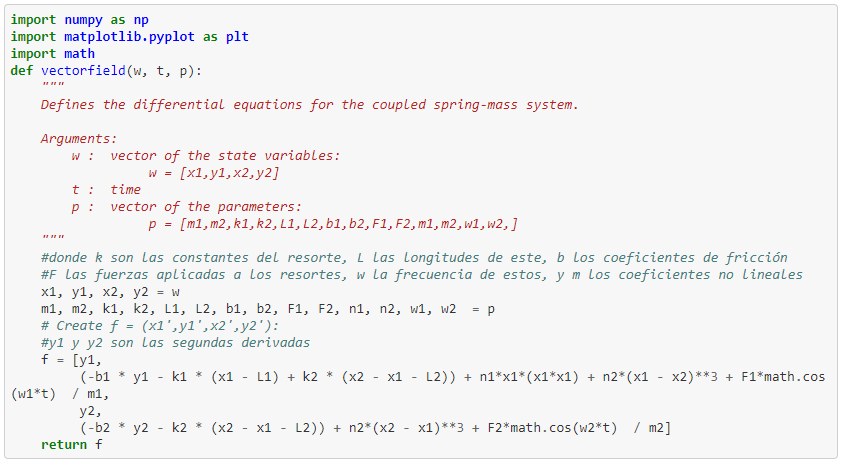
\includegraphics[width=1\textwidth]{Celda5.PNG}
    \centering
    \label{Cod}
\end{figure}

Las otros fragmentos de codigo mostrados en esta sección no sufrieron cambios.

\section {Ejemplos a resolver}
En las siguientes imágenes se pueden ver los ejemplos que se nos pedía resolver a lo largo de la actividad.
\begin{figure}[H]
    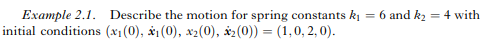
\includegraphics[width=1\textwidth]{Ejemplo2-1.PNG}
    \centering
    \label{Cod}
\end{figure}
\begin{figure}[H]
    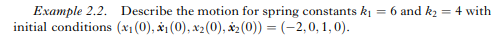
\includegraphics[width=1\textwidth]{Ejemplo2-2.PNG}
    \centering
    \label{Cod}
\end{figure}
\begin{figure}[H]
    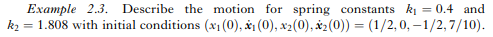
\includegraphics[width=1\textwidth]{Ejemplo2-3.PNG}
    \centering
    \label{Cod}
\end{figure}
\begin{figure}[H]
    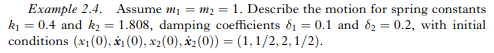
\includegraphics[width=1\textwidth]{Ejemplo2-4.PNG}
    \centering
    \label{Cod}
\end{figure}
\begin{figure}[H]
    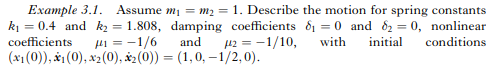
\includegraphics[width=1\textwidth]{Ejemplo3-1.PNG}
    \centering
    \label{Cod}
\end{figure}
\begin{figure}[H]
    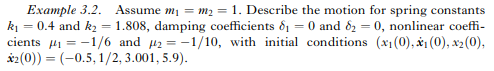
\includegraphics[width=1\textwidth]{Ejemplo3-2.PNG}
    \centering
    \label{Cod}
\end{figure}
\begin{figure}[H]
    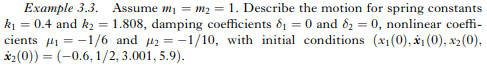
\includegraphics[width=1\textwidth]{Ejemplo3-3.PNG}
    \centering
    \label{Cod}
\end{figure}
\begin{figure}[H]
    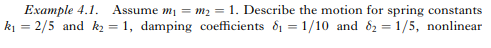
\includegraphics[width=1\textwidth]{Ejemplo4-1-1.PNG}
    \centering
    \label{Cod}
\end{figure}
\begin{figure}[H]
    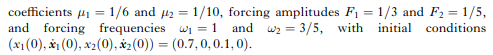
\includegraphics[width=1\textwidth]{Ejemplo4-1-2.PNG}
    \centering
    \label{Cod}
\end{figure}
\section{Resultados}
En primer lugar, se mostrará la gráfica obtenida a partir del código mostrado en la figura 3. En esta gráfica se puede apreciar el comportamiento del sistema de resorte-masa.
\begin{figure}[H]
    \caption{Gráfica 1 ejemplo 2.1}
    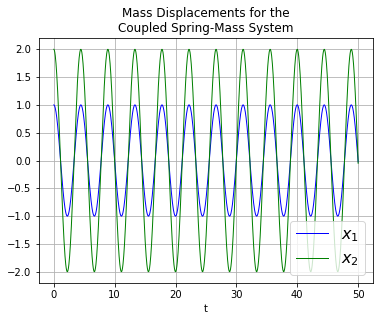
\includegraphics[width=0.5\textwidth]{Grafica1.png}
    \centering
    \label{Cod}
\end{figure}
En seguida, se muestra otro fragmento de código, el cual fue utilizado para obtener una gráfica que mostrará los retratos de fase de x1 y x2.
\begin{figure}[H]
    \caption{Celda 4}
    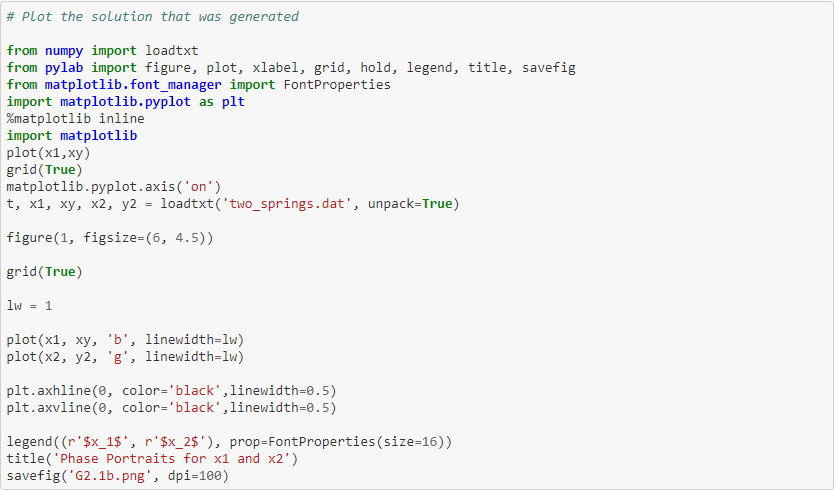
\includegraphics[width=1\textwidth]{Celda4.PNG}
    \centering
    \label{Cod}
\end{figure}
Esta sección de código, genero la siguiente gráfica:
\begin{figure}[H]
    \caption{Gráfica 2 ejemplo 2.1}
    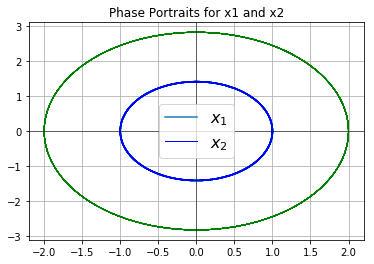
\includegraphics[width=0.5\textwidth]{Grafica2.png}
    \centering
    \label{Cod}
\end{figure}
La siguiente gráfica muestra el comportamiento de x1 contra x2:
\begin{figure}[H]
    \caption{Gráfica 3 ejemplo 2.1}
    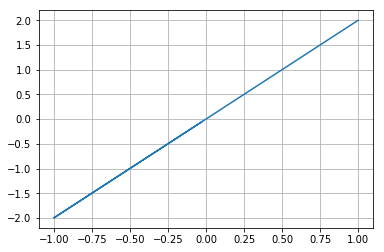
\includegraphics[width=0.5\textwidth]{Grafica3.png}
    \centering
    \label{Cod}
\end{figure}
Ahora, comparando las gráficas obtenidas mediante Jupyter Lab, con las gráficas mostradas en el archivo de texto, las cuales se muestra en la figura 8.
Se puede apreciar que en este caso las gráficas obtenidas mediante la solución númerica son las mismas que las obtenidas mediante la solución teoríca del archivo de texto.
\begin{figure}[H]
    \caption{Gráficas del ejemplo 2.1}
    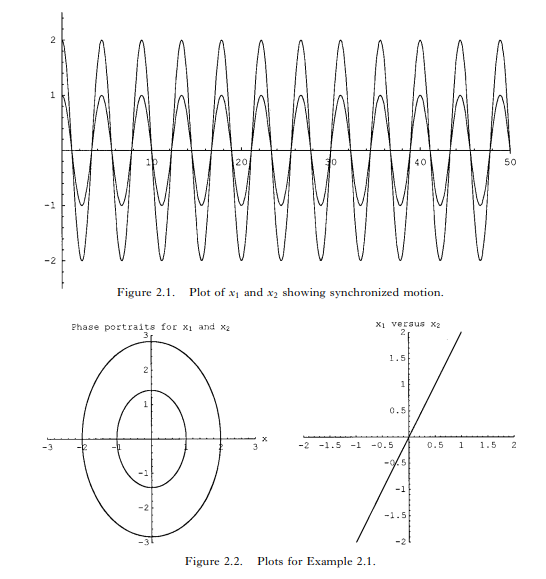
\includegraphics[width=0.5\textwidth]{Ejemplo1.PNG}
    \centering
    \label{Cod}
\end{figure}

Siguiendo con los resultados obtenidos para el ejemplo 2.2, se mostrarán sus gráficas, ya que para obtenerlas se utilizaron los mismos códigos mostrados con anterioridad, cambiando únicamente los datos númericos.
\begin{figure}[H]
    \caption{Gráfica 1 del ejemplo 2.2}
    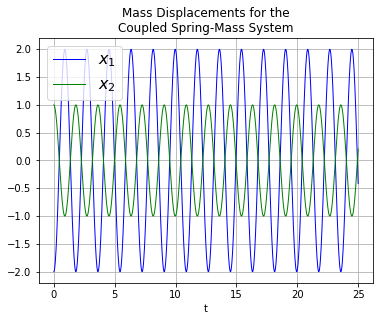
\includegraphics[width=0.5\textwidth]{Grafica4.png}
    \centering
    \label{Cod}
\end{figure}
Como en el ejemplo anterior, esta primera gráfica representa el comportamiento del sistema resorte-masa, mostrando en distintos colores el comportamiento de la elongación del resorte uno y del resorte dos.
A continuación se muestra la gráfica del comportamiento de x1 contra x2 para este ejemplo:
\begin{figure}[H]
    \caption{Gráfica 2 del ejemplo 2.2}
    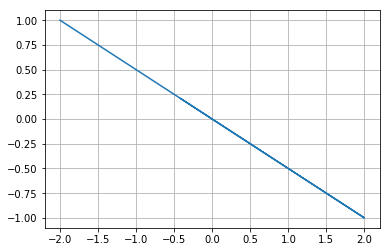
\includegraphics[width=0.5\textwidth]{Grafica5.png}
    \centering
    \label{Cod}
\end{figure}
Así como en el caso anterior, se puede ver que hay un comportamiento lineal entre ambas, sin embargo, en este ejemplo la pendiente mostrada es de carácter negativo, mientras que en el ejemplo 1 era de carácter positivo. Así como para el ejemplo anterior, también compararemos las gráficas obtenidas con la solución númerica con las esperadas del archivo de texto.
\begin{figure}[H]
    \caption{Gráficas del ejemplo 2.2}
    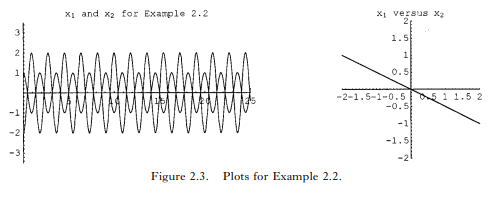
\includegraphics[width=1\textwidth]{Ejemplo2.PNG}
    \centering
    \label{Cod}
\end{figure}
Comparando las gráficas obtenidas con las esperadas, se puede ver que son básicamente las mismas, lo que me lleva a pensar que la solución númerica obtenida esta bastante cercana a la solución teórica.

Ahora, pasamos a las gráficas obtenidas para los datos del ejemplo 2.3, como en los casos anteriores se presentará primero la gráfica del comportamiento del sistema resorte-masa
\begin{figure}[H]
    \caption{Gráfica 1 del ejemplo 2.3}
    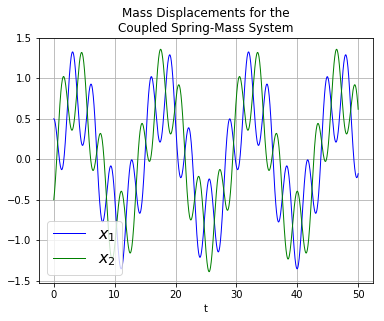
\includegraphics[width=0.5\textwidth]{Grafica6.png}
    \centering
    \label{Cod}
\end{figure}
Para este caso, el comportamiento del sistema es ligeramente diferente a los casos anteriores, esto puede deberse a que sus condiciones son bastante diferentes a como lo fueron en los casos anteriores, no obstante, aún puede verse el comportamiento oscilatorio del sistema.
La figura 13 nos mostrará una gráfica del comportamiento de x1, con respecto a su primera derivada. Mientras que la figura 14 nos mostrará el comportamiento de x2 con respecto a su derivada también.
\begin{figure}[H]
    \caption{Gráfica 2 del ejemplo 2.3}
    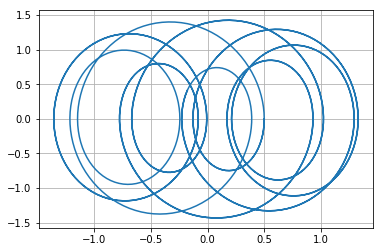
\includegraphics[width=0.5\textwidth]{Grafica7.png}
    \centering
    \label{Cod}
\end{figure}
\begin{figure}[H]
    \caption{Gráfica 3 del ejemplo 2.3}
    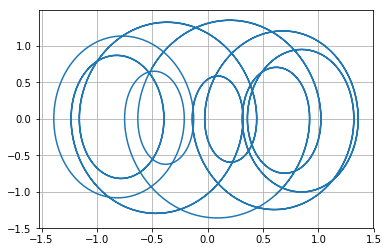
\includegraphics[width=0.5\textwidth]{Grafica8.png}
    \centering
    \label{Cod}
\end{figure}
Por último, se presenta la gráfica del comportamiento de x1 contra x2.
\begin{figure}[H]
    \caption{Gráfica 4 del ejemplo 2.3}
    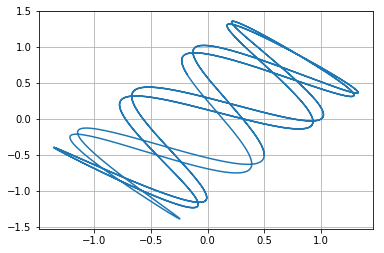
\includegraphics[width=0.5\textwidth]{Grafica9.png}
    \centering
    \label{Cod}
\end{figure}
Comparando las gráficas obtenidas con las esperadas, notamos una ligera diferencia en las gráficas de los comportamientos de x1 y x2 con respecto a sus derivadas, mientras que las gráficas de x1 contra x2, y la del comportamiento oscilatorio del sistema son las mismas
\begin{figure}[H]
    \caption{Gráficas del ejemplo 2.3}
    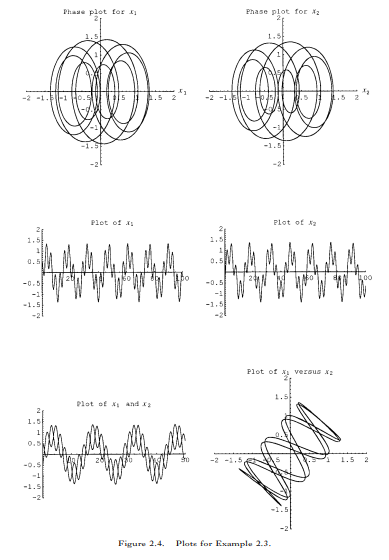
\includegraphics[width=0.5\textwidth]{Ejemplo3.PNG}
    \centering
    \label{Cod}
\end{figure}

Por último las gráficas del ejemplo 2.4, como en los casos anteriores se mostrará primero la gráfica del comportamiento oscilatorio del sistema:
\begin{figure}[H]
    \caption{Gráfica 1 del ejemplo 2.4}
    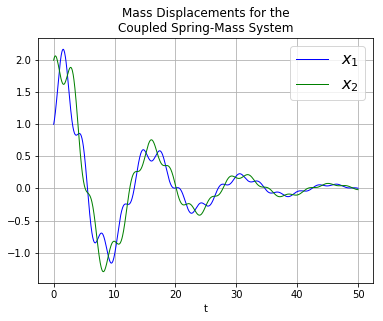
\includegraphics[width=0.5\textwidth]{Grafica10.png}
    \centering
    \label{Cod}
\end{figure}
La siguiente figura muestra el comportamiento de x1 contra x2, siendo en esta ocasión un movimiento un tanto más difícil de explicar, ya que, a diferencia de los casos anteriores, se tiene un movimiento que se puede considerar asimétrico y "no cerrado" como en el ejemplo 2.3
\begin{figure}[H]
    \caption{Gráfica 2 del ejemplo 2.4}
    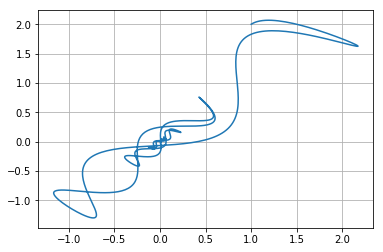
\includegraphics[width=0.5\textwidth]{Grafica11.png}
    \centering
    \label{Cod}
\end{figure}
Las siguientes figuras muestran los comportamientos de x1 y x2 con sus respectivas derivadas, en el mismo orden que se mencionan.
\begin{figure}[H]
    \caption{Gráfica 2 del ejemplo 2.4}
    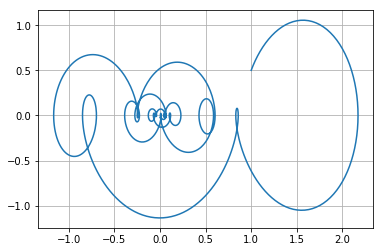
\includegraphics[width=0.5\textwidth]{Grafica12.png}
    \centering
    \label{Cod}
\end{figure}
\begin{figure}[H]
    \caption{Gráfica 3 del ejemplo 2.4}
    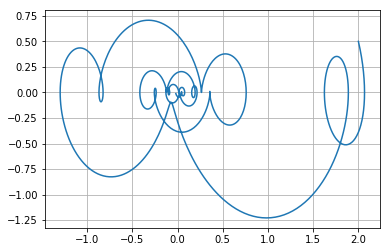
\includegraphics[width=0.5\textwidth]{Grafica13.png}
    \centering
    \label{Cod}
\end{figure}
En el caso de los comportamientos de x1 y x2 con sus respectivas derivadas, podemos decir lo mismo que se dijo anteriormente sobre la gráfica del comportamiento de x1 contra x2, que no hay simetría en sus movimientos.
Para finalizar con esta parte, compararemos las gráficas obtenidas con las gráficas esperadas:
\begin{figure}[H]
    \caption{Gráficas del ejemplo 2.4}
    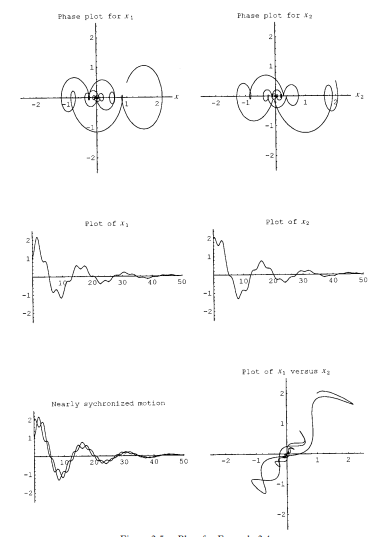
\includegraphics[width=0.5\textwidth]{Ejemplo4.PNG}
    \centering
    \label{Cod}
\end{figure}
Comparando estas las gráficas obtenidas por medio de la solución númerica, y las esperadas del archivo de texto, podemos ver que se tratan de las mismas, es decir, como en los casos de los ejemplos anteriores, se obtuvieron los mismos resultados de la solución esperada.

Continuando con las gráficas del ejemplo 3.1, tenemos la siguiente para el comportamiento del sistema resorte-masa.
\begin{figure}[H]
    \caption{Gráfica 1 del ejemplo 3.1}
    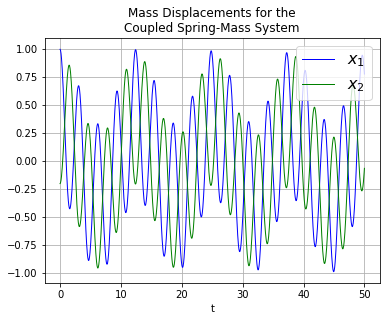
\includegraphics[width=0.5\textwidth]{Grafica14.png}
    \centering
    \label{Cod}
\end{figure}
Como en los primeros casos del ejercicio 2, se puede apreciar un comportamiento simétrico en las vibraciones del sistema.
A continuación la gráfica del comportamiento de x1 con respecto a x2
\begin{figure}[H]
    \caption{Gráfica 2 del ejemplo 3.1}
    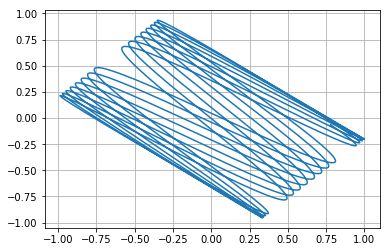
\includegraphics[width=0.5\textwidth]{Grafica15.png}
    \centering
    \label{Cod}
\end{figure}
Y las gráficas de x1 y x2 con respecto a sus derivadas, en el mismo orden que se mencionan:
\begin{figure}[H]
    \caption{Gráfica 3 del ejemplo 3.1}
    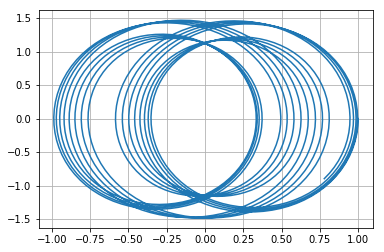
\includegraphics[width=0.5\textwidth]{Grafica16.png}
    \centering
    \label{Cod}
\end{figure}
\begin{figure}[H]
    \caption{Gráfica 4 del ejemplo 3.1}
    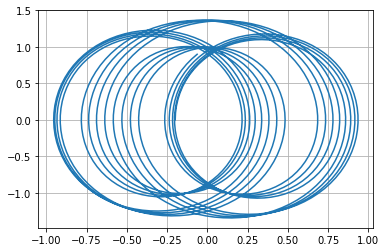
\includegraphics[width=0.5\textwidth]{Grafica17.png}
    \centering
    \label{Cod}
\end{figure}
Estas dos últimas figuras muestran diferencia con las gráficas esperadas del archivo de texto, como podemos ver con la siguiente imagen:
\begin{figure}[H]
    \caption{Gráficas del ejemplo 3.1}
    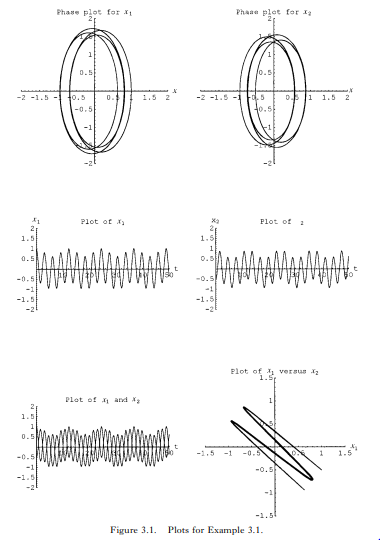
\includegraphics[width=0.5\textwidth]{Ejemplo5.PNG}
    \centering
    \label{Cod}
\end{figure}
Las obtenidas por medio de la solución númerica se ven más circulares que las esperadas, no obstante, el comportamiento de las otras dos gráficas es el mismo en las gráficas obtenidas que en las esperadas.
Continuando con el ejemplo 3.2, se obtuvo la siguiente gráfica para el comportamiento del sistema:
\begin{figure}[H]
    \caption{Gráfica 1 del ejemplo 3.2}
    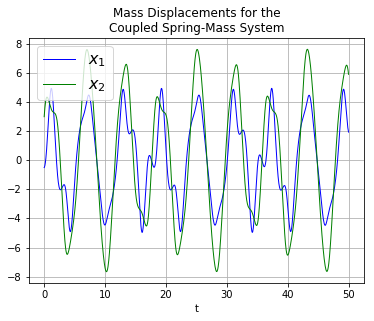
\includegraphics[width=0.5\textwidth]{Grafica18.png}
    \centering
    \label{Cod}
\end{figure}
La siguiente figura muestra la gráfica para el comportamiento de x1 contra x2:
\begin{figure}[H]
    \caption{Gráfica 2 del ejemplo 3.2}
    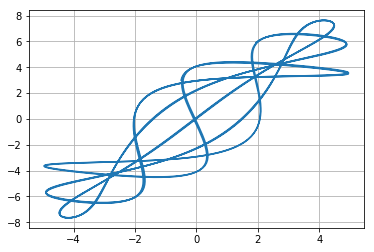
\includegraphics[width=0.5\textwidth]{Grafica19.png}
    \centering
    \label{Cod}
\end{figure}
Y los comportamientos de x1 y x2 con respecto a sus derivadas, en el orden mencionado
\begin{figure}[H]
    \caption{Gráfica 3 del ejemplo 3.2}
    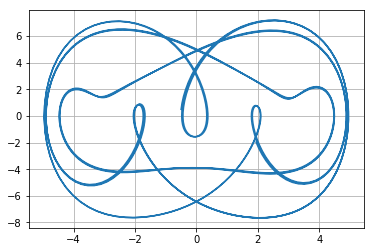
\includegraphics[width=0.5\textwidth]{Grafica20.png}
    \centering
    \label{Cod}
\end{figure}
\begin{figure}[H]
    \caption{Gráfica 4 del ejemplo 3.2}
    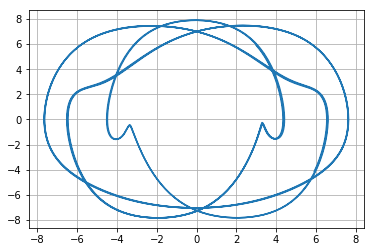
\includegraphics[width=0.5\textwidth]{Grafica21.png}
    \centering
    \label{Cod}
\end{figure}
Las gráficas obtenidas para este ejemplo coinciden con las gráficas esperadas en la solución del archivo de texto, como se puede ver con la siguiente figura
\begin{figure}[H]
    \caption{Gráficas del ejemplo 3.2}
    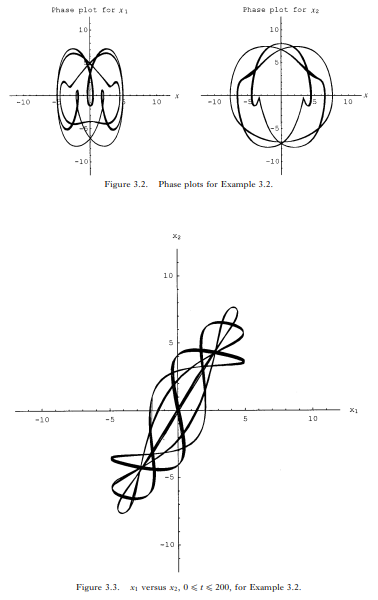
\includegraphics[width=0.5\textwidth]{Ejemplo6.PNG}
    \centering
    \label{Cod}
\end{figure}

Siguiendo con el ejemplo 3.3, se presenta la gráfica obtenida para el comportamiento del sistema:
\begin{figure}[H]
    \caption{Gráfica 1 del ejemplo 3.3}
    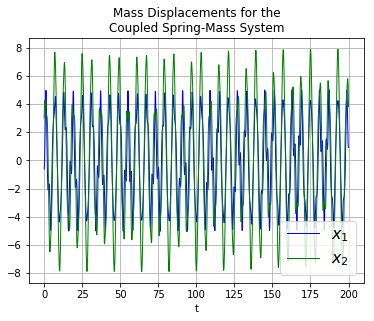
\includegraphics[width=0.5\textwidth]{Grafica22.png}
    \centering
    \label{Cod}
\end{figure}
La gráfica del comportamiento de x1 contra  x2 es la siguiente:
\begin{figure}[H]
    \caption{Gráfica 2 del ejemplo 3.3}
    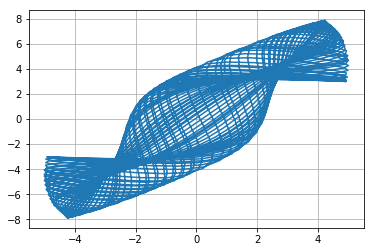
\includegraphics[width=0.5\textwidth]{Grafica23.png}
    \centering
    \label{Cod}
\end{figure}
Y las representaciones gráficas del comportamiento de x1 y x2 con sus respectivas derivadas:
\begin{figure}[H]
    \caption{Gráfica 3 del ejemplo 3.3}
    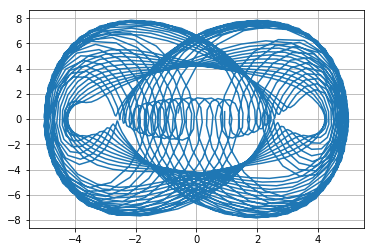
\includegraphics[width=0.5\textwidth]{Grafica24.png}
    \centering
    \label{Cod}
\end{figure}
\begin{figure}[H]
    \caption{Gráfica 4 del ejemplo 3.3}
    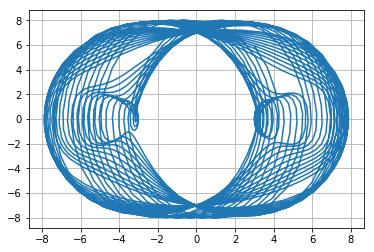
\includegraphics[width=0.5\textwidth]{Grafica25.png}
    \centering
    \label{Cod}
\end{figure}
Estas gráficas son bastante similares a las esperadas, en realidad podría decirse que son las mismas, aunque con una diferencia en la cantidad de puntos que conforman las curvas que describen el movimiento del sistema, esto se puede comprobar con la siguiente figura
\begin{figure}[H]
    \caption{Gráficas del ejemplo 3.3}
    \includegraphics[width=0.5\textwidth]{Ejemplo7.PNG}
    \centering
    \label{Cod}
\end{figure}

Para finalizar con esta sección, se presentaran las gráficas obtenidas para el ejemplo 4.1
\begin{figure}[H]
    \caption{Gráfica 1 del ejemplo 4.1}
    \includegraphics[width=0.5\textwidth]{Grafica26.png}
    \centering
    \label{Cod}
\end{figure}
El comportamiento de x1 contra x2 en este sistema:
\begin{figure}[H]
    \caption{Gráfica 2 del ejemplo 4.1}
    \includegraphics[width=0.5\textwidth]{Grafica29.png}
    \centering
    \label{Cod}
\end{figure}
Y el comportamiento de x1 y x2 contra sus respectivas derivadas:
\begin{figure}[H]
    \caption{Gráfica 3 del ejemplo 4.1}
    \includegraphics[width=0.5\textwidth]{Grafica27.png}
    \centering
    \label{Cod}
\end{figure}
\begin{figure}[H]
    \caption{Gráfica 4 del ejemplo 4.1}
    \includegraphics[width=0.5\textwidth]{Grafica28.png}
    \centering
    \label{Cod}
\end{figure}
Estas gráficas son ligeramente diferentes a las esperadas, como lo podemos ver mediante las siguientes dos figuras:
\begin{figure}[H]
    \caption{Gráficas del ejemplo 4.1}
    \includegraphics[width=0.5\textwidth]{Ejemplo8.PNG}
    \centering
    \label{Cod}
\end{figure}
\begin{figure}[H]
    \includegraphics[width=0.5\textwidth]{Ejemplo8-1.PNG}
    \centering
    \label{Cod}
\end{figure}
Esta diferencia que existe entre las gráficas que se obtuvieron y las que se esperaban, puede deberse al método con el que se soluciono el problema.

\section{Conclusiones}
Los métodos númericos para resolver ecuaciones diferenciales, entre otras ecuaciones matemáticas, son una herramienta bastante útil y poderosa, la cual los físicos debemos empezar a dominar para poder emplearlas cómodamente en nuestro trabajo, ya que facilitan la obtención de resultados, que por otros métodos quizás no seríamos capaces de obtener.

\section{Bibliografía}
\begin{enumerate}
\item Temple H Fay, S. D. (2002). coupled springs equations. En T. H. Fay, Coupled Springs Equations (pág. 16).
\item Weckesser, W. (17 de 02 de 2018). SciPhy Cookbook. Obtenido de http://scipy-cookbook.readthedocs.io/items/CoupledSpringMassSystem.html
\end {enumerate}
 
\section{Ápendice}
\begin{itemize}
\item ¿Qué más te llama la atención de la actividad completa?, ¿qué se te hizo menos interesante? \\ creo que lo que más llama la atención es el como resolver el problema y como modificar las ecuaciones para poder emplearlas en el código
\item ¿De un sistema de masas acopladas como se trabaja en esta actividad, hubieras pensado que abre toda una nueva área de fenómenos no lineales? \\ No lo habría considerado muy a fondo, probablemente habría pensando que habría mucho material con que trabajar si se consideraban fuerzas externas y de fricción, sin embargo, no me hubiera detenido demasiado a pensar en ello
\item ¿Qué propondrías para mejorar esta actividad?, ¿te ha parecido interesante este reto? \\ En definitiva fue un reto interesante
\item ¿Quisieras estudiar más este tipo de fenómenos no lineales? \\ Creo que estaría bien estudiarlos un poco más, ya que en la mayoría de los casos nos enfrentaremos a problemas no lineales
\end{itemize}
\end{document}
